\documentclass[11pt,letterpaper]{book}

\usepackage{times}
%-------------------------
% the following magic makes the tt font in math mode be the same as the
% normal tt font (i.e., Courier)
%
\SetMathAlphabet{\mathtt}{normal}{OT1}{pcr}{n}{n}
\SetMathAlphabet{\mathtt}{bold}{OT1}{pcr}{bx}{n}
%-------------------------

\usepackage[top=1.33in, bottom=1.33in, left=1.33in, right=1.33in]{geometry}
\usepackage{amsmath}
\usepackage[all]{xy}
\usepackage{graphicx}
\usepackage{stmaryrd}

\newcommand{\ulex}{\texttt{ml-ulex}}
\newcommand{\mlantlr}{\texttt{ml-antlr}}
\newcommand{\antlr}{\texttt{ml-antlr}}
\newcommand{\Antlr}{\texttt{Ml-antlr}}

\title{
  SML/NJ Language Processing Tools:\\
  User Guide}
\author{
  Aaron Turon\\
  \texttt{adrassi@gmail.com}\\[0.5em]
  John Reppy\\
  \texttt{jhr@cs.chicago.edu}}
\date{Revised: October 2020}

\newcommand{\Carat}{\^{ }}
\newcommand{\RE}{r}
\newcommand{\OR}{\ | \ }
\newcommand{\AND}{\ \& \ }
\newcommand{\CL}{\mathcal{L}}
\newcommand{\CS}{\mathcal{S}}
\newcommand{\CR}{\mathcal{R}}
\newcommand{\CP}{\mathcal{P}}
\newcommand{\Sem}[1]{[ \! [ #1 ] \! ]}
\newcommand{\Ls}[1]{\CL\Sem{#1}}

\newcommand{\eg}{{\em e.g.}}
\newcommand{\cf}{{\em cf.}}
\newcommand{\ie}{{\em i.e.}}

\newcommand{\nm}[1]{\texttt{#1}}

\newcommand{\ra}{\rightarrow}
\newcommand{\Ra}{\Rightarrow}

\newcommand{\New}[1]{\emph{\textbf{#1}}}

% Grammar
\newcommand{\Grammar}[1]{\[ \begin{array}{rcll} #1 \end{array} \]}
\newcommand{\GFirst}[3]{#1 & ::= & #2 & \textrm{#3} \\ }
\newcommand{\GNext}[2]{ & | & #1 & \textrm{#2} \\ }

\newcommand{\GFirstB}[2]{\textit{#1} & ::= & \multicolumn{2}{l}{\textit{#2}} \\ }
\newcommand{\GNextB}[1]{ & | & \multicolumn{2}{l}{\textit{#1}} \\ }

\newcommand{\GFirstC}[3]{\textit{#1} & ::= & \textit{#2} & \textrm{#3} \\ }
\newcommand{\GNextC}[2]{ & | & \textit{#1} & \textrm{#2} \\ }
\newcommand{\GNextCC}[2]{ & | & \multicolumn{2}{l}{\textit{#1}} \\ & & & \textrm{#2} \\ }

%\newcommand{\T}[1]{{\tt '#1'}}
\newcommand{\T}[1]{{\textbf{\tt #1}}}
\newcommand{\kw}[1]{{\T{\%#1}}}

\usepackage{amsthm}

\newtheorem*{theorem}{Theorem}
\newtheorem*{definition}{Definition}
\newtheorem*{remark}{Remark}

\usepackage{ifpdf}

\usepackage{mathpazo}
%\renewcommand{\ttdefault}{cmtt}

%\newcommand{\parttext}{}
%\newcommand{\cpart}[1]{\renewcommand{\parttext}{#1}\part{#1}}

\usepackage{fancyhdr}
\usepackage{multicol}

\newcommand{\sem}[1]{\llbracket #1\rrbracket}

\usepackage{color}
\definecolor{Red}{rgb}{0.9,0.0,0.0}
\definecolor{DarkBlue}{rgb}{0.0,0.0,0.75}
\definecolor{Purple}{rgb}{0.5,0.0,0.4}
\definecolor{DarkGreen}{rgb}{0.0,0.5,0.0}
\newcommand{\cdColor}{DarkBlue}
\newcommand{\kwColor}{Purple}
\newcommand{\dirColor}{Purple}
\newcommand{\strColor}{DarkGreen}
\newcommand{\comColor}{Red}

\usepackage{listings}

\lstdefinelanguage{SML}{%
  morekeywords={%
    abstype, and, andalso, as, case, datatype, do, else, end, eqtype, exception,%
    fn, fun, functor, handle, if, in, include, infix, infixr, let, local, nonfix,%
    of, op, open, orelse, raise, rec, sharing, sig, signature, struct, structure,%
    then, type, val, where, while, with, withtype%
  },%
  otherkeywords={[,],\{,\},\,,:,...,_,|,=,=>,->,\#,:>},
  sensitive,%
  alsoletter={_},
  morecomment=[n]{(*}{*)},%
  morestring=[d]",%
}[keywords,comments,strings]%

\lstdefinelanguage{CM}{%
  morekeywords={%
    functor, signature, structure,%
    Library, is,%
  },%
  sensitive,%
  alsoletter={_},
  morecomment=[n]{(*}{*)},%
  morestring=[d]",%
}[keywords,comments,strings]%

\lstdefinelanguage{MLULex}[]{SML}{%
  moredirectives={arg,defs,header,let,name,states},
  moredelim=*[directive]\%,%
  alsoletter={_},
}[keywords,comments,strings,directives]%

\lstdefinelanguage{MLAntlr}{%
  morekeywords={\%defs,\%entry,\%header,\%import,\%keywords,\%name,\%nonterms,of,
    \%refcell,\%tokens,\%tokentype,\%start,\%value},
  sensitive,%
  alsoletter={_,\%},%
  morecomment=[n]{(*}{*)},%
  morestring=[d]",%
}[keywords,comments,strings]%

\lstset{
  basicstyle=\footnotesize\ttfamily\color{\cdColor},
  keywordstyle=\color{\kwColor}\bfseries,
  commentstyle=\color{\comColor}\itshape,
  directivestyle=\color{\dirColor}\bfseries,
  stringstyle=\color{\strColor}\itshape,
  showstringspaces=false,
  language=SML
}

\begin{document}

\frontmatter

	\maketitle
	
	\phantom{.}
	\vspace{\stretch{1}}
	
	\noindent Copyright \copyright{}2016.  Fellowship of SML/NJ.  All rights reserved.
	
	\vskip 12pt
	\noindent This document was written with support. in part, from NSF grant
	CNS-0454136, ``CRI: Standard ML Software Infrastructure.''
	
	\pagebreak
	
	\tableofcontents

\mainmatter

%	\renewcommand{\chaptermark}[1]{\markboth{#1}{}}
%	\renewcommand{\sectionmark}[1]{\markright{\thesection. \ #1}{}}

	\newpage

	\chapter{Overview}\label{chap:overview}

In software, language recognition is ubiquitous: nearly every program deals at some level with structured input given in textual form.  The simplest recognition problems can be solved directly, but as the complexity of the language grows, recognition and processing become more difficult.  

Although sophisticated language processing is sometimes done by hand, the use of scanner and parser generators\footnote{
  ``Scanner generator'' and ``parser generator'' will often be shortened to ``scanner'' and ``parser'' respectively.  This is justified by viewing a parser generator as a parameterized parser.
} is more common.  The Unix tools {\tt lex} and {\tt yacc} are the archetypical examples of such generators.  Tradition has it that when a new programming language is introduced, new scanner and parser generators are written in that language, and generate code for that language.  Traditional \emph{also} has it that the new tools are modeled after the old {\tt lex} and {\tt yacc} tools, both in terms of the algorithms used, and often the syntax as well.  The language Standard ML is no exception: {\tt ml-lex} and {\tt ml-yacc} are the SML incarnations of the old Unix tools.

This manual describes two new tools, \ulex{} and \mlantlr{}, that follow tradition in separating scanning from parsing, but break from tradition in their implementation: \ulex{} is based on \emph{regular expression derivatives} rather than subset-construction, and \mlantlr{} is based on $LL(k)$ parsing rather than $LALR(1)$ parsing.   

\section{Motivation}

Most parser generators use some variation on $LR$ parsing, a form of \emph{bottom-up} parsing that tracks possible interpretations (reductions) of an input phrase until only a single reduction is possible.  While this is a powerful technique, it has the following downsides:
\begin{itemize}
  \item Compared to predictive parsing, it is more complicated and difficult to understand.  This is particularly troublesome when debugging an $LR$-ambiguous grammar.
  \item Because reductions take place as late as possible, the choice of reduction cannot depend on any semantic information; such information would only become available \emph{after} the choice was made.
  \item Similarly, information flow in the parser is strictly bottom-up.  For (syntactic or semantic) context to influence a semantic action, higher-order programming is necessary.
\end{itemize} 
The main alternative to $LR$ parsing is the top-down, $LL$ approach, which is commonly used for hand-coded parsers.  An $LL$ parser, when faced with a decision point in the grammar, utilizes lookahead to unambiguously predict the correct interpretation of the input.  As a result, $LL$ parsers do not suffer from the problems above.  $LL$ parsers have been considered impractical because the size of their prediction table is exponential in $k$ --- the number of tokens to look ahead --- and many languages need $k > 1$.  However, Parr showed that an approximate form of lookahead, using tables linear in $k$, is usually sufficient.

To date, the only mature $LL$ parser based on Parr's technique is his own parser, {\tt antlr}.  While {\tt antlr} is sophisticated and robust, it is designed for and best used within imperative languages.  The primary motivation for the tools this manual describes is to bring practical $LL$ parsing to a functional language.
Our hope with \ulex{} and \mlantlr{} is to modernize and improve the Standard ML language processing infrastructure, while demonstrating the effectiveness of regular expression derivatives and $LL(k)$ parsing.  The tools are more powerful than their predecessors, and they raise the level of discourse in language processing.  

%\section{Outline}

%This manual is organized into three parts: usage, theory, and implementation.  Each of these parts is further broken down into two chapters, one on \ulex{} and one on \mlantlr{}.  The usage section is self-contained, and gives a fairly complete specification of the two tools.  Full details on the algorithms used are given in the theory section.  Data structures, system organization, and other code-related particulars are described in the implementation section.
	
%	\renewcommand{\chaptermark}[1]{\markboth{\parttext{}: #1}{}}

%	\cpart{Usage}
	
		%!TEX root = manual.tex
%
\chapter{ML-ULex}

%\section{Overview}

Lexers analyze the lexical structure of an input string, and are usually specified using regular expressions.  \textsc{ml-ulex} is a lexer generator for Standard ML.  The module it generates will contain a type \texttt{strm} and a function
\begin{verbatim}
    val lex : AntlrStreamPos.sourcemap -> strm
          -> lex_result * AntlrStreamPos.span * strm
\end{verbatim}%
where \texttt{lex\char`\_result} is a type that must be defined by the user of \ulex{}.
Note that the lexer always returns a token: we assume that end-of-file will be explicitly represented by a token.
Compared to ML-Lex, \ulex{} offers the following improvements:
\begin{itemize}
 \item Unicode is supported under the UTF8 encoding.
 \item Regular expressions can include intersection and negation operators.
 \item The position span of a token is automatically computed and returned to the lexer's caller (as can be seen
   by the specification of the \texttt{lex} function above).
 \item The specification format is somewhat cleaner.
 \item The code base is much cleaner, and supports multiple back-ends, including DFA graph visualization and interactive testing of rules.
\end{itemize}%
The tool is invoked from the command-line as follows:
\begin{verbatim}
    ml-ulex [options] file
\end{verbatim}%
where \texttt{file} is the name of the input \ulex{} specification, and where \texttt{options} may be any combination of:

\vskip 12pt
\begin{tabular}{lp{0.65\textwidth}}
  \texttt{--dot} & generate DOT output (for graphviz; see \texttt{http://www.graphviz.org}).  The produced file will be named \texttt{file.dot}, where \texttt{file} is the input file. \\
  \\
  \texttt{--match} & enter interactive matching mode.  This will allow interactive testing of the machine; presently, only the \texttt{INITIAL} start state is available for testing
  (see Section~\ref{sec:start-states} for details on start states).  \\
  \\
  \texttt{--ml-lex-mode} & operate in \texttt{ml-lex} compatibility mode.  See Section~\ref{sec:lex-compat} for details. \\
  \\
  \texttt{--table-based} & generate a table-based lexer.\\
  \\
  \texttt{--fn-based} & generate a lexer that represents states as functions and transitions as tail calls.\\
  \\
  \texttt{--minimize} & generate a minimal machine.  Note that this is slow, and is almost never necessary. \\
  \\
  \texttt{--strict-sml} & generate strict SML (\ie{}, do not use SML/NJ extensions).  This flag
    is useful if you want to use the output with a different SML system.
\end{tabular}

\vskip 10pt \noindent
The output file will be called \texttt{file.sml}.

\section{Specification format}

A \ulex{} specification is a list of semicolon-terminated \emph{declarations}.  Each declaration is either a \emph{directive} or a \emph{rule}.  Directives are used to alter global specification properties (such as the name of the module that will be generated) or to define named regular expressions.  Rules specify the actual reguluar expressions to be matched.  The grammar is given in Figure~\ref{fig:ulex-syntax}.

\begin{figure}
\Grammar{
\GFirstB{spec}
	{$($ declaration \T{;} $)^*$}

\GFirstB{declaration}
	{directive}
\GNextB
	{rule}

%	{\kw{charset} $($ \T{ASCII7} $|$ \T{ASCII8} $|$ \T{UTF8} $)$}

\GFirstB{directive}
	{\kw{arg} code}
\GNextB
	{\kw{defs} code}
\GNextB
	{\kw{let} ID \T{=} re}
\GNextB
	{\kw{name} ID}
\GNextB
	{\kw{header} code}
\GNextB
	{\kw{states} ID$^+$}
	
\GFirstB{code}
	{ \T{(} $\dots$ \T{)} }
	
\GFirstB{rule}
	{ $($\T{<} ID $($ \T{,} ID $)^*$ \T{>}$)^?$ re \T{=>} code}
\GNextB
	{ $($\T{<} ID $($ \T{,} ID $)^*$ \T{>}$)^?$ \T{<<EOF>>} \T{=>} code}

\GFirstB{re}
	{CHAR}
\GNextB
	{\T{"} SCHAR$^*$ \T{"}}
\GNextB
	{\T{(} re \T{)}}
\GNextCC
	{\T{[} $($ \T{-} $|$ \T{\^{ }} $)^?$ $($ CCHAR \T{-} CCHAR $|$ CCHAR $)^+$ 
	 \T{-}$^?$ \T{]} \quad\phantom{.}}
				{a character class}
\GNextC
	{\T{\{} ID \T{\}}}	{\kw{let}-bound RE}
\GNextC
	{\T{.}}			{wildcard (any single character including \texttt{{$\backslash$}n})}
\GNextC
	{re \T{*}}		{Kleene-closure (0 or more)}
\GNextC
	{re \T{?}}		{optional (0 or 1)}
\GNextC
	{re \T{+}}		{positive-closure (1 or more)}
\GNextC
	{re \T{\{} NUM \T{\}}}	{exactly {\it NUM} repetitions}
\GNextC
	{re \T{\{} NUM$_1$, \ NUM$_2$ \T{\}}}	{between {\it NUM$_1$} and {\it NUM$_2$} repetitions}
\GNextC
	{re re}			{concatenation}
\GNextC
	{\T{$\sim$} re}	{negation} %(any string not matched by \textit{re})}
\GNextC
	{re \T{\&} re}	{intersection}
\GNextC
	{re \T{|} re}	{union}
%\GNextB
%	{re \T{/} re}
%\GNextB
%	{re \T{\$}}
%\GNextB
%	{\T{\_}}
\GFirstB{CHAR}
	{any printable character not one of \ 
		$\begin{array}[t]{l}
		\normalfont
		 \texttt{\^{ } < > $\backslash$ ( ) \{ \} [ \& | * ?}\\
		\normalfont
		 \texttt{+ " . ; = $\sim$ }
		 \end{array}$}
\GNextB{an SML or Unicode escape code}
\GFirstB{CCHAR}
	{any printable character not one of \ \T{\^{ } - ] $\backslash$}}
\GNextB{an SML or Unicode escape code}
\GFirstB{SCHAR}
	{any printable character not one of \ \T{" $\backslash$}}
\GNextB{an SML or Unicode escape code}
\GFirstB{NUM}
	{one or more digits}
}
\caption{The \ulex{} grammar}\label{fig:ulex-syntax}
\end{figure}

There are a few lexical details of the specification format worth mentioning.  First, SML-style comments (\texttt{(* ... *)}) are treated as ignored whitespace anywhere they occur in the specification, \emph{except} in segments of code.  The \textit{ID} symbol used in the grammar stands for alpha-numeric-underscore identifiers, starting with an alpha character.  The \textit{code} symbol represents a segment of SML code, enclosed in parentheses.  Extra parentheses occuring within strings or comments in code need not be balanced.

A complete example specification appears in Chapter~\ref{ch:example}.

\section{Directives}

\subsection{The \kw{arg} directive}

Specifies an additional curried parameter, appearing after the sourcemap parameter, that will be passed into the \texttt{lex} function and made available to all lexer actions.

\subsection{The \kw{defs} directive}

The \kw{defs} directive is used to include a segment of code in the generated lexer module, as in the following example:
\begin{lstlisting}
%defs (
  type lex_result = CalcParseToks.token
  fun eof() = CalcParseTokens.EOF
  fun helperFn x = (* ... *)
)
\end{lstlisting}
The definitions must at least fulfill the following signature:
\begin{lstlisting}
type lex_result
val eof : unit -> lex_result
\end{lstlisting}
unless EOF rules are specified, in which case only the \texttt{lex\char`\_result} type is needed~(see Section~\ref{sec:eof-rules}).
All semantic actions must yield values of type \texttt{lex\char`\_result}.  The \texttt{eof} function is called by \ulex{} when the end of file is reached -- it acts as the semantic action for the empty input string.  All definitions given will be in scope for the rule actions (see Section~\ref{sec:ulex-rules}).

\subsection{The \kw{let} directive}

Use \kw{let} to define named abbreviations for regular expressions; once bound, an abbreviation can be used in further \kw{let}-bindings or in rules.  For example,
\begin{verbatim}
%let digit = [0-9];
\end{verbatim}
introduces an abbreviation for a regular expression matching a single digit.  To use abbreviations, enclose their name in curly braces.  For example, an additional \kw{let} definition can be given in terms of \texttt{digit},
\begin{verbatim}
%let int = {digit}+;
\end{verbatim}
which matches arbitrary-length integers.  Note that scoping of let-bindings follows standard SML rules, so that the definition of \texttt{int} must appear after the definition of \texttt{digit}.

\subsection{The \kw{name} directive}

The name to use for the generated lexer module is specified using \kw{name}.

\subsection{The \kw{header} directive}
The \kw{header} directive allows one to specify the lexer's header.
This directive is useful when you want to use a functor for the lexer.
For example,
\begin{lstlisting}
%header (functor ExampleLexFn (Extras : EXTRA_SIG));
\end{lstlisting}%
Note that it is an error to include both the \kw{header} and \kw{name} directive in the
same lexer specification.

\subsection{The \kw{states} directive}
\label{sec:start-states}

It is often helpful for a lexer to have multiple \emph{start states}, which influence
the regular expressions that the lexer will match. 
For instance, after seeing a double-quote, the lexer might switch into a \texttt{STRING}
start state that contains only the rules necessary for matching strings, and which
returns to the standard start state after the closing quote.

Start states are introduced via \kw{states} and are named using standard identifiers. 
There is always an implicit, default start state called \texttt{INITIAL}.
Within a rule action, the function \texttt{YYBEGIN} can be applied to the name
of a start state to switch the lexer into that state; see~\ref{sec:ulex-actions}
for details on rule actions.

Using start states allows the lexer to be defined as a collection of finite-state machines
(one per start state), with arbitrary SML code used to control switching between machines.
This mechanism thus allows non-regular features to be supported by the lexer, such as
nested comments.

\section{Rules}\label{sec:ulex-rules}

In general, when \texttt{lex} is applied to an input stream, it will attempt to match a prefix of the input with a regular expression given in one of the rules.  When a rule is matched, its \emph{action} (associated code) is evaluated and the result is returned.  Hence, all actions must belong to the same type. %, but no restrictions are placed on what that type is.
Rules are specified by an optional list of start states, a regular expression, and the action code.  The rule is said to ``belong'' to the start states it lists.  If no start states are specified, the rule belongs to \emph{all} defined start states.

Rule matching is determined by three factors: start state, match length, and rule order.  A rule is only considered for matching if it belongs to the lexer's current start state.  If multiple rules match an input prefix, the rule matching the longest prefix is selected.  In the case of a tie, the rule appearing first in the specification is selected.

For example, suppose the start state \texttt{FOO} is defined, and the following rules appear, with no other rules belonging to \texttt{FOO}:
\begin{verbatim}
    <FOO> a+    => ( Tokens.as );
    <FOO> a+b+  => ( Tokens.asbs );
    <FOO> a+bb* => ( Tokens.asbs );
\end{verbatim}
If the current start state is not \texttt{FOO}, none of the rules will be considered.  Otherwise, on input ``aabbbc'' all three rules are possible matches.  The first rule is discarded, since the others match a longer prefix.  The second rule is then selected, because it matches the same prefix as the third rule, but appears earlier in the specification.

\subsection{Regular expression syntax}

\newcommand{\REX}{\textit{re}}
\begin{figure}
\begin{minipage}[t]{.5\textwidth}
\begin{eqnarray*}
  \sem{\T{.}} &=& \Sigma \\
  \sem{\REX_1 \ \REX_2} &=& \sem{\REX_1} \cdot \sem{\REX_2} \\
  \sem{\T{$\sim$} \ \REX} &=& \left(\bigcup_{i=0}^\infty \Sigma^i\right)\setminus \sem{\REX} \\
  \sem{\REX_1 \ \T{\&} \ \REX_2} &=& \sem{\REX_1} \cap \sem{\REX_2} \\
  \sem{\REX_1 \ \T{|} \ \REX_2} &=& \sem{\REX_1} \cup \sem{\REX_2} \\
  \sem{\REX \ \T{?}} &=& \sem{\REX} \cup \{ \epsilon \}
\end{eqnarray*}
\end{minipage}\begin{minipage}[t]{.5\textwidth}
\begin{eqnarray*}
  \sem{\REX \ \T{*}} &=& \bigcup_{i=0}^\infty \sem{\REX}^i \\
  \sem{\REX \ \T{+}} &=& \bigcup_{i=1}^\infty \sem{\REX}^i \\
  \sem{\REX \ \T{\{} n \T{\}}} &=& \sem{\REX}^n \\
  \sem{\REX \ \T{\{} n \T{, } m \T{\}}} &=& \bigcup_{i=n}^m \sem{\REX}^i
\end{eqnarray*}
\end{minipage}
\caption{Semantics for regular expressions}\label{ulex-re-semantics}
\end{figure}

The syntax of regular expressions is given in Figure~\ref{fig:ulex-syntax}; constructs are listed in precedence order, from most tightly-binding to least.  Escape codes are the same as in SML, but also include \texttt{$\backslash$uxxxx} and \texttt{$\backslash$Uxxxxxxxx}, where \texttt{xxxx} represents a hexidecimal number which in turn represents a Unicode symbol.  The specification format itself freely accepts Unicode characters, and they may be used within a quoted string, or by themselves.

The semantics for \ulex{} regular expressions are shown in Figure~\ref{ulex-re-semantics}; they are standard.  Some examples:
\[
\begin{array}{rcl}
\texttt{0 | 1 | 2 | 3}	& \textit{denotes} &
    \{ \texttt{0}, \texttt{1}, \texttt{2}, \texttt{3} \}	\\
\texttt{[0123]}	& \textit{denotes} &
    \{ \texttt{0}, \texttt{1}, \texttt{2}, \texttt{3} \}	\\
\texttt{0123}	& \textit{denotes} &
    \{ \texttt{0123} \}						\\
\texttt{0*}	& \textit{denotes} &
    \{ \epsilon, \texttt{0}, \texttt{00}, \dots \}		\\
\texttt{00*}	& \textit{denotes} &
    \{ \texttt{0}, \texttt{00}, \dots \}		\\
\texttt{0+}	& \textit{denotes} &
    \{ \texttt{0}, \texttt{00}, \dots \}		\\
\texttt{[0-9]\{3\}}	& \textit{denotes} &
    \{ \texttt{000}, \texttt{001}, \texttt{002}, \dots, \texttt{999} \}	\\
\texttt{0* \& (..)*}	& \textit{denotes} &
    \{ \epsilon, \texttt{00}, \texttt{0000}, \dots \}	\\
\texttt{\^{ }(abc)}	& \textit{denotes} &
    \Sigma^* \setminus \{ \texttt{abc} \}	\\
\texttt{[\^{ }abc]}	& \textit{denotes} &
    \Sigma \setminus \{ \texttt{a}, \texttt{b}, \texttt{c} \}
\end{array}
\]

\subsection{EOF rules}\label{sec:eof-rules}

It is sometimes useful for the behavior of a lexer when it reaches the end-of-file to change
depending on the current start state.
Normally, there is a single user-defined \texttt{eof} function that defines EOF behavior, but
EOF rules can be used to be more selective, as in the following example:
\begin{verbatim}
  <INITIAL> <<EOF>> => ( Tok.EOF );
  <COMMENT> <<EOF>> => ( print "Error: unclosed comment";
                         Tok.EOF );
\end{verbatim}
Other than the special \T{<<EOF>>} symbol, EOF rules work exactly like normal rules.

Note that if you define any EOF rules, then you must define EOF rules for all states;
otherwise, your scanner may generate a \texttt{Match} exception on EOF.
Furthermore, if you define EOF rules, you do not need a definition of the \texttt{eof}
function.

\subsection{Actions}\label{sec:ulex-actions}

\newcommand{\itemtt}[2]{\item[{\normalfont\textbf{\texttt{val}} \texttt{#1} \texttt{:} \texttt{#2}}]\mbox{}\\}

Actions are arbitrary SML code enclosed in parentheses.  The following names are in scope:
\begin{description}
  \itemtt{YYBEGIN}{yystart\char`\_state -> unit}
    This function changes the start state to its argument.
  \itemtt{yysetStrm}{ULexBuffer.stream -> unit}
    This function changes the current input source to its argument.
    The functions \texttt{yystreamify}, \texttt{yystreamifyInstream} and \texttt{yystreamifyReader}
    can be used to construct the stream; they work identically to the corresponding functions
    described in Section~\ref{sec:ulex-code}
  \itemtt{yytext}{string}
    The matched text as a string.
  \itemtt{yysubstr}{substring}
    The matched text as a substring (avoids copying).
  \itemtt{yyunicode}{UTF8.wchar list}
    The matched text as a list of Unicode wide characters (\ie{}, words).
  \itemtt{continue}{unit -> lex\char`\_result}
    This function recursively calls the lexer on the input following the matched prefix, and returns its result.
    The span for the resulting token begins at the left border of the match that calls \texttt{continue}.
  \itemtt{skip}{unit -> lex\char`\_result}
    This function is identical to \texttt{continue}, except that it moves forward the left marker
    for the span of the returned token.
    For example, \texttt{skip} can be used to skip preceding whitespace.
  \itemtt{yysm}{AntlrSourcePos.sourcemap}
    the sourcemap for the lexer, to be used with the functions in the \texttt{AntlrSourcePos} module.
  \itemtt{yypos}{ref int}
    the input character position of the left border of the matched RE, starting from 0.
  \itemtt{yylineno}{ref int}
    The current line number, starting from 1.
    Note that lines are counted using the Unix line-ending convention.
  \itemtt{yycolno}{ref int}
    The current column number, starting from 1.
\end{description}%
Futhermore, any name bound in the \kw{\%defs} section is in scope in the actions.

\section{Using the generated code}\label{sec:ulex-code}

The generated lexer module has a signature that includes the following specifications:
\begin{lstlisting}
type prestrm
type strm = prestrm * start_state
    
val streamify         : (unit -> string) -> strm
val streamifyReader   : (char, 'a) StringCvt.reader -> 'a -> strm
val streamifyInstream : TextIO.instream -> strm
    
val lex : AntlrStreamPos.sourcemap -> strm
      -> lex_result * AntlrStreamPos.span * strm
\end{lstlisting}%
where \texttt{lex\char`\_result} is the result type of the lexer actions, and \texttt{start\char`\_state} is an algebraic datatype with nullary constructors for each defined start state.
Note that \texttt{lex\char`\_result} must be defined as a type using the \kw{defs} directive.
In this interface, lexer start states are conceptually part of the input stream; thus, from an external viewpoint,
start states can be ignored.
It is, however, sometimes helpful to control the lexer start state externally, allowing contextual
information to influence the lexer.
This is why the \texttt{strm} type includes a concrete \texttt{start\char`\_state} component.

Note that the \texttt{AntlrStreamPos} module is part of the \texttt{ml-lpt-lib} library described in Chapter~\ref{ch:ml-lpt-lib}. 
An \texttt{AntlrStreamPos.sourcemap} value, combined with an \texttt{AntlrStreamPos.pos} value, compactly represents position information (line number, column number, and so on).
An \texttt{AntlrStreamPos.span} is a pair of \texttt{pos} values that specify the character position of the
leftmost (first) character of the scanned token and the position of the
rightmost (last) character in the token (respectively).
By default, the span will cover the entire sequence of characters consumed by a call to the lexer, but one may
use the \texttt{skip} function (see Section~\ref{sec:ulex-actions}) to ignore leading whitespace,
\textit{etc.}\ when computing the span.
Code to compute the span is generated automatically by \texttt{ml-ulex}.

\section{\texttt{ml-lex} compatibility}\label{sec:lex-compat}

Running \ulex{} with the \texttt{--ml-lex-mode} option will cause it to process its input file using the ML-Lex format, and interpret the actions in a ML-Lex-compatible way.  The compatibility extends to the bugs in ML-Lex, so in particular \texttt{yylineno} starts at 2 in \texttt{--ml-lex-mode}.

		%!TEX root = manual.tex
%
\chapter{ML-Antlr}

%\section{Overview}

Parsers analyze the syntactic structure of an input string, and are usually specified with some variant of context-free grammars.  \antlr{} is a parser generator for Standard ML based on Terence Parr's variant of $LL(k)$ parsing.  The details of the parsing algorithm are given in the companion implementation notes; the practical restrictions on grammars are discussed in Section~\ref{sec:antlr-llk}.  A parser generated by \antlr{} is a functor; it requires a module with the \texttt{ANTLR\char`\_LEXER} signature:
\begin{lstlisting}
signature ANTLR_LEXER = sig
    type strm
    val getPos : strm -> AntlrStreamPos.pos
  end
\end{lstlisting}
Applying the parser functor will yield a module containing a \texttt{parse} function:
\begin{lstlisting}
val parse : 
      (Lex.strm -> ParserToks.token * AntlrStreamPos.span * Lex.strm)
        -> Lex.strm
          -> result_ty option * strm * ParserToks.token AntlrRepair.repair list
\end{lstlisting}
where \texttt{result\char`\_ty} is determined by the semantic actions for the parser.  The \texttt{ParserTokens} module is generated by \antlr{} (see Section~\ref{sec:antlr-gencode}) and the \texttt{AntlrRepair} module is available in the \texttt{ml-lpt} library (see Chapter~\ref{ch:ml-lpt-lib}). 

Notable features of \antlr{} include:
\begin{itemize}
 \item Extended BNF format, including Kleene-closure (*), positive closure (+), and optional (?) operators.
 \item Robust, automatic error repair.
 \item Selective backtracking.
 \item ``Inherited attributes'': information can flow downward as well as upward during a parse.
 \item Semantic predicates: a syntactic match can be qualified by a semantic condition.
 \item Grammar inheritence.
 \item Convenient default actions, especially for EBNF constructions.
 \item Convenient abbreviations for token names (\emph{e{.}g{.}}, \texttt{"("} rather than \texttt{LP})
\end{itemize}
The tool is invoked from the command-line as follows:
\begin{verbatim}
    ml-antlr [options] file
\end{verbatim}
where \texttt{file} is the name of the input \ulex{} specification, and where \texttt{options} may be any combination of:

\vskip 12pt
\begin{tabular}{lp{0.65\textwidth}}
  \texttt{--dot} & generate DOT output (for graphviz; see \texttt{http://www.graphviz.org}).
    The generated file will be named \texttt{file.dot}, where \texttt{file} is the input file. \\
  \\
  \texttt{--latex} & generate a simple \LaTeX version of the grammar, named \texttt{file.tex}. \\
  \\
  \texttt{--unit-actions} & ignore the action code in the grammar, and instead return \texttt{()}
    for every production. \\
  \\
  \texttt{--debug} & add code to the actions to print the left-hand-side of the production.
\end{tabular}%

\vskip 10pt \noindent
The output file will be called \texttt{file.sml}.

\section{Background definitions}

Before describing \antlr{}, we need some terminology.  A \emph{context-free grammar} (CFG) is a set of \emph{token} (or \emph{terminal}) symbols, a set of \emph{nonterminal} symbols, a set of \emph{productions}, and a start symbol $S$, which must be a nonterminal.  
The general term \emph{symbol} refers to both tokens and nonterminals.  A production relates a nonterminal $A$ to a string of symbols $\alpha$; we write this relation as $A \ra \alpha$.  Suppose $\alpha A \beta$ is a symbol string, and $A$ is a nonterminal symbol.  We write $\alpha A \beta \Ra \alpha \gamma \beta$ if $A \ra \gamma$ is a production; this is called a one-step derivation.  In general, a CFG generates a language, which is a set of token strings.  The strings included in this language are exactly those token string derived in one or more steps from the start symbol $S$.

A parser recognizes whether an input string is in the language generated by a given CFG, usually computing some value (such as a parse tree) while doing so.  The computations performed during a parse are called \emph{semantic actions} (or just \emph{actions}).

\section{Specification format}\label{sec:antlr-spec}

A \antlr{} specification is a list of semicolon-terminated \emph{declarations}.  Each declaration is either a \emph{directive} or a \emph{nonterminal definition}.  Directives are used to alter global specification properties (such as the name of the functor that will be generated) or to define supporting infrastructure for the grammar.  The nonterminal definitions specify the grammar itself.  The grammar for \antlr{} is given in Figure~\ref{fig:antlr-syntax}.

\begin{figure}
\Grammar{
\GFirstB{spec}
	{$($ declaration \T{;} $)^*$}

\GFirstB{declaration}
	{directive}
\GNextB
	{nonterminal}

\GFirstB{directive}
	{\kw{defs} code}
\GNextB
	{\kw{entry} ID $($ \T{,} ID $)^*$}
\GNextB
	{\kw{import} STRING $($ \kw{dropping} symbol$^+$ $)^?$}
\GNextB
	{\kw{keywords} symbol $($ \T{,} symbol $)^*$}
\GNextB
	{\kw{value} ID code}
\GNextB
	{\kw{name} ID}
\GNextB
	{\kw{header} code}
\GNextB
	{\kw{refcell} ID \T{:} monotype \T{=} code}
\GNextB
	{\kw{start} ID}
\GNextB
	{\kw{tokentype} qualid}
\GNextB
	{\kw{tokens} \T{:} tokdef $($ \T{|} tokdef $)^*$}
\GNextB
	{\kw{nonterms} \T{:} datacon $($ \T{|} datacon $)^*$}
	
\GFirstB{code}
	{ \T{(} $\dots$ \T{)} }

\GFirstB{tokdef}
	{datacon $($ \T{(} STRING \T{)} $)^?$}

\GFirstB{datacon}
	{ID}
\GNextB
	{ID \T{of} monotype}

\GFirstB{nonterminal}
	{ID formals$^?$ \T{:} prodlist}

\GFirstB{formals}
	{ \T{(} ID $($ \T{,} ID $)^*$ \T{)} }
	
\GFirstB{prodlist}
	{production $($ \T{|} production $)^*$}
	
\GFirstB{production}
	{\kw{try}$^?$ named-item$^*$ $($ \kw{where} code $)^?$ $($ \T{=>} code $)^?$ }
\GFirstB{named-item}
	{$($ ID \T{:} $)^?$ item}
\GFirstB{item}
	{prim-item \T{?}}
\GNextB
	{prim-item \T{+}}
\GNextB
	{prim-item \T{*}}
	
\GFirstB{prim-item}
	{symbol $($ \T{@} code $)^?$}
\GNextB
	{ \T{(} prodlist \T{)} }

\GFirstB{symbol}
	{ID}
\GNextB
	{STRING}

\GFirstB{monotype}{\textrm{An SML monomorphic type expression}}
	
\GFirstB{qualid}{\textrm{An SML qualified identifier}}

\GFirstB{ID}{\textrm{An SML identifier}}
\GFirstB{STRING}{\textrm{An SML string literal}}
}
\caption{The \antlr{} grammar}\label{fig:antlr-syntax}
\end{figure}

SML-style comments (\texttt{(* ... *)}) are treated as ignored whitespace anywhere they occur in the specification, \emph{except} in segments of code.  The \textit{code} symbol represents a segment of SML code, enclosed in parentheses.  Extra parentheses occuring within strings or comments in code need not be balanced.
A complete example specification appears in Chapter~\ref{ch:example}.

Most \antlr{} declarations are \emph{cumulative}: they may appear multiple times in a grammar specification, with each new declaration adding to the effect of the previous ones.  Thus, for instance, the specification fragment
\begin{lstlisting}[language=MLAntlr]
    %tokens : foo ;
    %tokens : bar of string ;
\end{lstlisting}%
is equivalent to the single directive
\begin{lstlisting}[language=MLAntlr]
    %tokens : foo | bar of string ;
\end{lstlisting}%
and similarly for nonterminal definitions and so on.  All declarations are cumulative except for the \kw{start} and \kw{name} directives.
The reason for treating specifications in this way is to give the \kw{import} directive very simple semantics, as described below.

\section{Directives}

\subsection{The \kw{defs} directive}

The \kw{defs} directive is used to include a segment of code in the generated parser:  
\begin{lstlisting}[language=SML]
%defs (
  fun helperFn x = (* ... *)
);
\end{lstlisting}%
All definitions given will be in scope for the semantic actions (see Section~\ref{sec:antlr-actions}).

\subsection{The \kw{entry} directive}

It is often useful to parse input based on some fragment of a grammar.  When a nonterminal is declared to be an \emph{entry point} for the grammar via \kw{entry}, \antlr{} will generate a separate \texttt{parse} function that expects the input to be a string derived from that nonterminal.  Given a grammar with a nonterminal \texttt{exp} and the declaration
\begin{lstlisting}[language=MLAntlr]
    %entry exp;
\end{lstlisting}%
the generated parser will include a function
\begin{lstlisting}
val parseexp : (Lex.strm -> ParserToks.token * AntlrStreamPos.span * Lex.strm)
      -> Lex.strm
        -> exp_ty option * strm * ParserToks.token AntlrRepair.repair list
\end{lstlisting}
where \texttt{exp\char`\_ty} is the type of the actions for the \texttt{exp} nonterminal.  Note that if \texttt{exp} has inherited attributes (Section~\ref{sec:inh-attr}) they will appear as a tuple argument, curried after the lexer argument:
\begin{lstlisting}
val parseexp : (Lex.strm -> ParserToks.token * AntlrStreamPos.span * Lex.strm)
      -> attributes
        -> Lex.strm
          -> exp_ty option * strm * ParserToks.token AntlrRepair.repair list
\end{lstlisting}
Finally, the \emph{start} symbol (Section~\ref{sec:start}) is always an entry point to the grammar, but the generated function is simply called \texttt{parse}.

\subsection{The \kw{import} directive}

The \kw{import} directive is used to include one grammar inside another.  The string given in the directive should hold the path to a grammar file, and $\backslash$ characters must be escaped.  By default, all declarations appearing in the specified file are included in the resulting grammar, except for \kw{start}, \kw{entry}, and \kw{name} declarations.  However, individual tokens or nonterminals can be dropped by listing them in the \kw{dropping} clause of an \kw{import} declaration.  Since nonterminal definitions are cumulative (Section~\ref{sec:antlr-nt}), the imported nonterminals can be extended with new productions simply by listing them.
The final grammar must, of course, ensure that all used tokens and nonterminals are defined.

\subsection{The \kw{keywords} and \kw{value} directives}

\Antlr{} uses an error-repair mechanism that is based on inserting or deleting tokens until
a correct parse is found.
The \kw{keywords} and \kw{default} directives allow one to improve this process.
Since changes to the input involving keywords can drastically alter the meaning of the
input, it is usually desirable to favor non-keyword repairs.
The \kw{keywords} directive is used to tell \antlr{} which tokens should be considered keywords.
The \kw{value} directive is used to define a default argument for non-nullary tokens, which
is used to construct a token value that can be inserted into the token stream
when attempting to find a repair.
For example
\begin{lstlisting}[language=MLAntlr]
    %value NUMBER(0);
\end{lstlisting}%
would allow the \texttt{NUMBER} token to be inserted as an error repair.

Section~\ref{sec:antlr-gencode} describes how to report error repairs to the user.
%When a syntax error is discovered, \antlr{} attempts to find a single-token repair to the input that will %allow the parse to continue.

\subsection{The \kw{name} directive}

The prefix to use for the name of the generated parser functor is specified using \kw{name}.
In addition to the functor, \antlr{} will generate a module to define the \texttt{token} datatype.
If the declaration
\begin{lstlisting}[language=MLAntlr]
    %name Example;
\end{lstlisting}%
appears in the specification, then the parser functor will be named
\texttt{ExampleParseFn} and the tokens module will be called \texttt{ExampleTokens}.

\subsection{The \kw{header} directive}
The \kw{header} directive allows one to specify the parser's functor.
This directive is useful when you want to add additional parameters to the functor,
but the declaration must include the \texttt{Lex} structure with signature
\texttt{ANTLR\char`\_LEXER}.
For example,
\begin{lstlisting}
%header (
  functor ExampleParseFn (
      structure Lex : ANTLR_LEXER
      structure Extras : EXTRA_SIG));
\end{lstlisting}%

\noindent{}\textbf{Note:} the \kw{header} directive was added in SML/NJ version 110.72.

\subsection{The \kw{refcell} directive}

Because semantic actions must be pure (for backtracking and error repair), they cannot make use of standard reference cells to communicate information.
Nonterminals may inherit attributes (Section~\ref{sec:inh-attr}), which allows information to flow downward, but in some cases flowing information this way can become extremely tedious.
For example, a data structure may only need to be updated at a single point in the grammar, but in order to properly thread this state through the grammar, an inherited attribute would have to be added and propagated through every nonterminal.

The \kw{refcell} directive is used to declare a backtracking-safe reference cell and make it available to all semantic actions.  Reference cells are declared by giving the name, type, and initial value for the cell.  Each cell is bound in the semantic actions as a standard SML \texttt{ref} value.  Thus, for example, we might have the following specification fragment:
\begin{lstlisting}[language=MLAntlr]
    %refcell symbols : StringSet.set = ( StringSet.empty );
    
    exp
      : INT
      | (exp)
      | ID => ( symbols := StringSet.add(!symbols, ID); ID )
      ;
\end{lstlisting}%
The result of this fragment is that all symbol uses are tracked, in any use of
the \texttt{exp} nonterminal, but without having to manually thread the data
structure state through the grammar.

The final contents of a reference cell is returned as an extra result from the parse
following the repair list.

\subsection{The \kw{start} directive}\label{sec:start}

A particular nonterminal must be designated as the start symbol for the grammar.  The start symbol can be specified using \kw{start}; otherwise, the first nonterminal defined is assumed to be the start symbol.

\subsection{The \kw{tokentype} directive}

As noted above, \mlantlr{} synthesizes a structure that contains a datatype representing the
tokens specified in the grammar.
In some situations, it may be useful to specify the token datatype elsewhere (\eg{}, if you
want to use the same lexer for two different parsers).
In such a case, one can use the \kw{tokentype} directive to give a qualified name for the token
dataype.
This identifier will be used in the tokens structure to specify the tokens type.
For example, if the grammar specification contains the directive
\begin{lstlisting}[language=MLAntlr]
    %tokentype MyTokens.t;
\end{lstlisting}%
then the code
\begin{lstlisting}[language=SML]
    datatype token = MyTokens.t
\end{lstlisting}%
in the tokens structure.
Even when the \kw{tokentype} directive is used, one must also declare the grammar's tokens
using the \kw{tokens} directive.
Furthermore, the user-supplied token datatype must include a nullary \texttt{EOF} constructor
in addition to exactly the constructors specified by the \kw{tokens} directives.\footnote{
  When the \kw{tokentype} directive is specified, \mlantlr{} will generate a signature for
  the tokens structure.
}

\noindent{}\textbf{Note:} the \kw{tokentype} directive was added in SML/NJ version 110.81.

\subsection{The \kw{tokens} directive}

The alphabet of the parser is defined using \kw{tokens}.  The syntax for this directive resembles a datatype declaration in SML, except that optional abbreviations for tokens may be defined.  For example:
\begin{lstlisting}[language=MLAntlr]
    %tokens
      : KW_let  ("let")  | KW_in   ("in")
      | ID of string     | NUM of Int.int
      | EQ      ("=")    | PLUS    ("+")
      | LP      ("(")    | RP      (")")
      ;
\end{lstlisting}%
Within nonterminal definitions, tokens may be referenced either by their name or abbreviation; the latter must always be double-quoted.

\subsection{The \kw{nonterms} directive}
\mlantlr{} normally identifies non-terminal symbols by their appearance on the left-hand side
of a production and relies on SML type inference to determine the type returned by parsing
a string derived from the nonterminal.
It is also possible to declare the type of a non-terminal using a \kw{nonterms} directive.

\section{Nonterminal definitions}\label{sec:antlr-nt}

The syntax of nontermal definitions is given in Figure~\ref{fig:antlr-syntax}.  As an illustration of the grammar, consider the following example, which defines a nonterminal with three productions, taking a formal parameter \texttt{env}:
\begin{lstlisting}[language=MLAntlr]
    atomicExp(env)
      : ID => ( valOf(AtomMap.find (env, Atom.atom ID)) )
      | NUM
      | "(" exp@(env) ")"
      ;
\end{lstlisting}%
Note that actions are only allowed at the end of a production, and that they are optional.

As with most directives, the non-terminal definitions are cumulative.
For example, the definition of \texttt{atomicExp} above could also be
written as three separate rules.
\begin{lstlisting}[language=MLAntlr]
    atomicExp(env) : ID => ( valOf(AtomMap.find (env, Atom.atom ID)) );
    atomicExp(env) : NUM;
    atomicExp(env) : "(" exp@(env) ")";
\end{lstlisting}%

\subsection{Extended BNF constructions}

In standard BNF syntax, the right side of a production is a simple string of symbols.  Extended BNF allows regular expression-like operators to be used: \texttt{*}, \texttt{+}, and \texttt{?} can follow a symbol, denoting 0 or more, 1 or more, or 0 or 1 occurrences respectively.  In addition, parentheses can be used within a production to enclose a \emph{subrule}, which may list several \texttt{|}-separated alternatives, each of which may have its own action.  In the following example, the nonterminal \texttt{item\char`\_list} matches a semicolon-terminated list of identifiers and integers:
\begin{lstlisting}[language=MLAntlr]
    item_list : (( ID | INT ) ";")* ;
\end{lstlisting}%
All of the extended BNF constructions have implications for the actions of a production; see Section~\ref{sec:antlr-actions} for details.

\subsection{Inherited attributes}\label{sec:inh-attr}

In most parsers, information can flow upward during the parse through actions, but not downard.  In attribute grammar terminology, the former refers to \emph{synthesized} attributes, while the latter refers to \emph{inherited attributes}.  Since \antlr{} is a predictive parser, it allows both kinds of attributes.  Inherited attributes are treated as parameters to nonterminals, which can be used in their actions or semantic predicates.  Formal parameters are introduced by enclosing them in parentheses after the name of a nonterminal and before its production list; the list of parameters will become a tuple.  In the following, the nonterminal \texttt{expr} takes a single parameter called \texttt{env}:
\begin{lstlisting}[language=MLAntlr]
    expr(env) : (* ... *) ;
\end{lstlisting}%
If a nonterminal has a formal parameter, any use of that nonterminal is required to apply it to an actual parameter.  Actual parameters are introduced in a production by giving the name of a nonterminal, followed by the \texttt{@} sign, followed by the code to compute the parameter.  For example:
\begin{lstlisting}[language=MLAntlr]
    assignment : ID ":=" expr@(Env.emptyEnv) ;
\end{lstlisting}%

\subsection{Selective backtracking}

Sometimes it is inconvenient or impossible to construct a nonterminal definition which can be unambiguously resolved with finite lookahead.
% (see Section~\ref{sec:antlr-llk} for examples).  
The \kw{try} keyword can be used to mark ambiguous \emph{productions} for selective backtracking.  For backtracking to take place, each involved production must be so marked.  Consider the following:
\begin{lstlisting}[language=MLAntlr]
    A : %try B* ";"
      | %try B* "(" C+ ")"
      ;
\end{lstlisting}%
As written, the two productions cannot be distinguished with finite lookahead, since they share an arbitrary long prefix of \texttt{B} nonterminal symbols.  Adding the \kw{try} markers tells \antlr{} to attempt to parse the first alternative, and if that fails to try the second.  Another way to resolve the ambiguity is the use of subrules, which do not incur a performance penalty:
\begin{lstlisting}[language=MLAntlr]
    A : B* ( ";"
           | "(" C+ ")"
           )
      ;
\end{lstlisting}%
This is essentially \emph{left-factoring}. See Section~\ref{sec:antlr-llk} for more guidance on working with the $LL(k)$ restriction.

\subsection{Semantic predicates}

A production can be qualified by a \emph{semantic predicate} by introducting a \kw{where} clause.  Even if the production is syntactically matched by the input, it will not be used unless its semantic predicate evaluates to \texttt{true}.  A \kw{where} clause can thus introduce context-sensitivity into a grammar.  The following example uses an inherited \texttt{env} attribute, containing a variable-value environment:
\begin{lstlisting}[language=MLAntlr]
    atomicExp(env)
      : ID %where ( AtomMap.inDomain(env, Atom.atom ID) )
           => ( valOf(AtomMap.find (env, Atom.atom ID)) )
      | NUM
      | "(" exp@(env) ")"
      ;
\end{lstlisting}%
In this example, if a variable is mentioned that has not been defined, the error is detected and reported during the parse as a syntax error.

Semantic predicates are most powerful when combined with selective backtracking.  The combination allows two syntactically identical phrases to be distinguished by contextual, semantic information.

\subsection{Actions}\label{sec:antlr-actions}

Actions for productions are just SML code enclosed in parentheses.  Because of potential backtracking and error repair, action code should be pure (except that they may update \antlr{} \texttt{refcell}s; see the \kw{refcell} directive).

In scope for an action are all the user definitions from the \kw{defs} directive.  In addition, the formal parameters of the production are in scope, as are the semantic yield of all symbols to the left of the action (the yield of a token is the data associated with that token's constructor).  In the following example, the first action has \texttt{env} and \texttt{exp} in scope, while the second action has \texttt{env} and \texttt{NUM} in scope:
\begin{lstlisting}[language=MLAntlr]
    atomicExp(env)
      : "(" exp@(env) ")" => ( exp )
      | NUM => ( NUM )
      ;
\end{lstlisting}%
Notice also that the actual parameter to \texttt{exp} in the first production is \texttt{env}, which is in scope at the point the parameter is given; \texttt{exp} itself would not be in scope at that point.

An important aspect of actions is naming: in the above example, \texttt{exp} and \texttt{NUM} were the default names given to the symbols in the production.  In general, the default name of a symbol is just the symbol's name.  If the same name appears multiple times in a production, a number is appended to the name of each yield, start from 1, going from left to right.  A subrule (any items enclosed in parentheses) is by default called \texttt{SR}.  Any default name may be overriden using the syntax \texttt{name=symbol}.  Overriding a default name does \emph{not} change the automatic number for other default names.  Consider:
\begin{lstlisting}[language=MLAntlr]
    foo : A bar=A A ("," A)* A*
        ;
\end{lstlisting}%
In this production, the names in scope from left to right are: \texttt{A1}, \texttt{bar}, \texttt{A3}, \texttt{SR}, \texttt{A4}.

The EBNF operators \texttt{*}, \texttt{+} and \texttt{?} have a special effect on the semantic yield of the symbols to which they are applied.  Both \texttt{*} and \texttt{+} yield a \emph{list} of the type of their symbol, while \texttt{?} yields an option.  For example, if \texttt{ID*} appeared in a production, its default name would be \texttt{ID}, and if the type of value of \texttt{ID} was \texttt{string}, it would yield a \texttt{string list}; likewise \texttt{ID?} would yield a \texttt{string option}.  

Subrules can have embedded actions that determine their yield:
\begin{lstlisting}[language=MLAntlr]
    plusList : ((exp "+" exp => ( exp1 + exp2 )) ";" => ( SR ))* => ( SR )
\end{lstlisting}%
The \texttt{plusList} nonterminal matches a list of semicolon-terminated additions.  The innermost subrule, containing the addition, yields the value of the addition; that subrule is contained in a larger subrule terminated by a semicolon, which yield the value of the inner subrule.  Finally, the semicolon-terminated subrule is itself within a subrule, which is repeated zero or more times.  Note that the numbering scheme for names is restarted within each subrule.

Actions are \emph{optional}: if an action is not specified, the default behavior is to return all nonterminals and non-nullary tokens in scope.  Thus, the last example can be written as 
\begin{lstlisting}[language=MLAntlr]
    plusList : ((exp "+" exp => ( exp1 + exp2 )) ";")*
\end{lstlisting}%
since \texttt{"+"} and \texttt{";"} represent nullary token values.

\section{The $LL(k)$ restriction}\label{sec:antlr-llk}

When working with any parser, one must be aware of the restrictions its algorithm places on grammars.
When \antlr{} analyzes a grammar, it attempts to create a prediction-decision
tree for each nonterminal.
In the usual case, this decision is made using lookahead token sets.  The tool will start with $k = 1$
lookahead and increment up to a set maximum until it can
uniquely predict each production.  Subtrees of the decision tree
remember the tokens chosen by their parents, and take this into account
when computing lookahead.  For example, suppose we have two productions
at the top level that generate the following sentences:
\begin{verbatim}
    prod1 ==> AA
    prod1 ==> AB
    prod1 ==> BC
    prod2 ==> AC
    prod2 ==> C
\end{verbatim}
At $k = 1$, the productions can generate the following sets:
\begin{verbatim}
    prod1 {A, B}
    prod2 {A, C}
\end{verbatim}
and $k = 2$,
\begin{verbatim}
    prod1 {A, B, C}
    prod2 {C, <EOF>}
\end{verbatim}
Examining the lookahead sets alone, this grammar fragment looks ambiguous
even for $k = 2$.  However, \antlr{} will generate the following decision
tree:
\begin{lstlisting}[language=SML]
if LA(0) = A then
  if LA(1) = A or LA(1) = B then
    predict prod1
  else if LA(1) = C then
    predict prod2
else if LA(0) = B then
  predict prod1
else if LA(1) = C then
  predict prod2
\end{lstlisting}%

In \antlr{}, only a small amount of lookahead is used by default ($k = 3$).  Thus, the following grammar is ambiguous for \antlr{}:
\begin{lstlisting}[language=MLAntlr]
    foo : A A A B
        | A A A A
        ;
\end{lstlisting}%
and will generate the following error message:
\begin{verbatim}
    Error: lookahead computation failed for 'foo',
    with a conflict for the following productions:
      foo ::= A A A A EOF
      foo ::= A A A B EOF
    The conflicting token sets are:
      k = 1: {A}
      k = 2: {A}
      k = 3: {A}
\end{verbatim}
Whenever a lookahead ambiguity is detected, an error message of this form is given.  The listed productions are the point of conflict.
The \texttt{k = ...} sets together give examples that can cause the ambiguity, in this case an input of \texttt{AAA}.

The problem with this example is that the two \texttt{foo} productions can only be distinguished by a token at $k = 4$ depth.  This situation can usually be resolved using \emph{left-factoring}, which lifts the common prefix of multiple productions into a single production, and then distinguishes the old productions through a subrule:
\begin{lstlisting}[language=MLAntlr]
    foo : A A A (B | A)
        ;
\end{lstlisting}%
Recall that subrule alternatives can have their own actions:
\begin{lstlisting}[language=MLAntlr]
    foo : A A A ( B => ( "got a B" ) 
                | A => ( "got an A" )
                )
        ;
\end{lstlisting}%
making left-factoring a fairly versatile technique.

Another limitation of predictive parsing is \emph{left-recursion}, where a nonterminal recurs without any intermediate symbols:
\begin{lstlisting}[language=MLAntlr]
    foo : foo A A
        | B
        ;
\end{lstlisting}%
Left-recursion breaks predictive parsing, because it is impossible to make a prediction for a left-recursive production without already having a prediction in hand.  Usually, this is quite easily resolved using EBNF operators, since left-recursion is most often used for specifying lists.  Thus, the previous example can be rewritten as
\begin{lstlisting}[language=MLAntlr]
    foo : B (A A)*
        ;
\end{lstlisting}%
which is both more readable and more amenable to $LL(k)$ parsing.

\section{Position tracking}

\antlr{} includes built-in support for propagating position information.  Because the lexer module is required to provide a \texttt{getPos} function, the tokens themselves do not need to carry explicit position information.
A position \emph{span} is a pair to two lexer positions (the type \texttt{AntlrStreamPos.span} is
an abbreviation for \texttt{AntlrStreamPos.pos * AntlrStreamPos.pos}).
Within action code, the position span of any symbol (token, nonterminal, subrule) is available as a value; if the yield of the symbol is named \texttt{Sym}, its span is called \texttt{Sym\char`\_SPAN}.
Note that the span of a symbol after applying the \texttt{*} or \texttt{+} operators is the
span of the entire matched list:
\begin{lstlisting}[language=MLAntlr]
    foo : A* => (* A_SPAN starts at the first A and ends at the last *)
\end{lstlisting}%
In addition, the span of the entire current production is available as \texttt{FULL\char`\_SPAN}.

%\section{Handling precedence}

\section{Using the generated code}\label{sec:antlr-gencode}

When \antlr{} is run, it generates a tokens module and a parser functor.
If the parser is given the name \texttt{Xyz} via the \kw{name} directive, these structures will be called \texttt{XyzParseFn} and \texttt{XyzTokens} respectively.  
The tokens module will contain a single datatype, called \texttt{token}.  The data constructors for the \texttt{token} type have the same name and type as those given in the \kw{tokens} directive; in addition, a nullary constructor called \texttt{EOF} will be available.

The generated parser functor includes the following:
\begin{lstlisting}[language=SML]
val parse : (Lex.strm -> ParserToks.token * AntlrStreamPos.span * Lex.strm)
      -> Lex.strm
        -> result_ty option * strm * ParserToks.token AntlrRepair.repair list
\end{lstlisting}%
where \texttt{result\char`\_ty} is the type of the semantic action for the grammar's start symbol.  
The \texttt{parse} function is given a lexer function and a stream.
The result of a parse is the semantic yield of the parse, the value of the stream at the end of the parse, and a list of error repairs.  
If an unrepairable error occurred, \texttt{NONE} is returned for the yield of the parse.

Note that if the start symbol for the grammar includes an inherited attribute (or a tuple of attributes), it will appear as an additional, curried parameter to the parser following the lexer parameter.  Suppose, for example, that a grammar has a start symbol with an inherited \texttt{Int.int AtomMap.map}, and that the grammar yields \texttt{Int.int} values.  The type of its \texttt{parse} function is as follows:
\begin{lstlisting}
    val parse : 
      (strm -> ParserToks.token * strm) -> 
      Int.int AtomMap.map -> 
      strm -> 
      Int.int option * strm * ParserToks.token AntlrRepair.repair list
\end{lstlisting}

The \texttt{AntlrRepair} module is part of the \texttt{ml-lpt-lib} library; it is fully described in Chapter~\ref{ch:ml-lpt-lib}.
It includes a function \texttt{repairToString}:
\begin{lstlisting}
val repairToString : 
      ('token -> string) -> AntlrStreamPos.sourcemap
        -> 'token repair -> string

\end{lstlisting}
which can be used to produce error messages from the parser's repair actions.
There is a more refined version of this function that allows one to specialize
the string representation of tokens based on whether the repair adds or deletes
them.
\begin{lstlisting}
datatype add_or_delete = ADD | DEL

val repairToString : 
      (add_or_delete -> 'token -> string) -> AntlrStreamPos.sourcemap
        ->'token repair -> string
\end{lstlisting}


Likewise, the tokens module (\texttt{ParserTokens} in this example) includes a function:
\begin{lstlisting}
val toString : token -> string
\end{lstlisting}
Thus, although error reporting is customizable, a reasonable default is provided, as illustrated below:
\begin{lstlisting}
let
  val sm = AntlrStreamPos.mkSourcemap()
  val (result, strm', errs) = Parser.parse (Lexer.lex sm) strm
  val errStrings = 
    map (AntlrRepair.repairToString ParserTokens.toString sm)
	errs
in
  print (String.concatWith "\n" errStrings)
end
\end{lstlisting}
The \texttt{toString} function will convert each token to its symbol as given in a \kw{tokens} directive,
using abbreviations when they are available.
By substituting a different function for \texttt{toString}, this behavior can be altered.

		%!TEX root = manual.tex
%
\chapter{The {\tt ml-lpt-lib} library}
\label{ch:ml-lpt-lib}

To use the output of \ulex{} or \mlantlr{} in an SML program requires including the
\texttt{ml-opt-lib} library.
This library includes the \texttt{AntlrStreamPos} structure, which manages tracking
positions in the input stream, and the \texttt{AntlrRepair} structure, which defines
a representation of \mlantlr{}'s error-repair actions that can be used to generate
error messages.

\section{Usage}
For SML/NJ, you should include the following line in your CM file:
\begin{lstlisting}[language=CM]
$/ml-lpt-lib.cm
\end{lstlisting}%
The SML/NJ Compilation Manager also understands how to generate SML files from \ulex{} and
\mlantlr{} files.
For example, if you include
\begin{lstlisting}
foo.grm : ml-antlr
foo.lex : ml-ulex
\end{lstlisting}%
in the list of sources in a CM file, then CM will run the \ulex{} (reps.\ \mlantlr{})
to produce \texttt{foo.lex.sml} (resp.\ \texttt{foo.grm.sml}).

If you are using MLton SML compiler, then you will need to include the following line
in your MLB file:
\begin{lstlisting}
$(SML_LIB)/mllpt-lib/mllpt-lib.mlb
\end{lstlisting}%

\section{The {\tt AntlrStreamPos} structure}

\begin{lstlisting}
structure AntlrStreamPos : sig

  type pos = int
  type span = pos * pos
  type sourceloc = { fileName : string option, lineNo : int, colNo : int }
  type sourcemap

  (* the result of moving forward an integer number of characters *)
  val forward : pos * int -> pos

  val mkSourcemap  : unit   -> sourcemap
  val mkSourcemap' : string -> sourcemap

  val same : sourcemap * sourcemap -> bool

  (* log a new line occurence *)
  val markNewLine : sourcemap -> pos -> unit
  (* resychronize to a full source location *)
  val resynch     : sourcemap -> pos * sourceloc -> unit

  val sourceLoc : sourcemap -> pos -> sourceloc
  val fileName  : sourcemap -> pos -> string option
  val lineNo    : sourcemap -> pos -> int
  val colNo     : sourcemap -> pos -> int
  val toString  : sourcemap -> pos -> string
  val spanToString : sourcemap -> span -> string

end
\end{lstlisting}%


\section{The {\tt AntlrRepair} structure}

\begin{lstlisting}
structure AntlrRepair : sig

  datatype 'tok repair_action
    = Insert of 'tok list
    | Delete of 'tok list
    | Subst of {
	old : 'tok list,
	new : 'tok list
      }
    | FailureAt of 'tok

  type 'a repair = AntlrStreamPos.pos * 'tok repair_action

  val actionToString :  ('tok -> string)
	-> 'tok repair_action
	-> string

  val repairToString : ('tok -> string)
	-> AntlrStreamPos.sourcemap
	-> 'tok repair -> string

  datatype add_or_delete = ADD | DEL

(* return a string representation of the repair action.  This version
 * uses the add_or_delete information to allow different token names
 * for deletion (more specific) and addition (more general).
 *)
  val actionToString' : (add_or_delete -> 'tok -> string)
	-> 'tok repair_action -> string
  val repairToString' : (add_or_delete -> 'tok -> string)
	-> AntlrStreamPos.sourcemap -> 'tok repair -> string

end
\end{lstlisting}%

		%!TEX root = manual.tex
%
\chapter{A complete example}
\label{ch:example}

This chapter gives a complete example of a simple calculator
language implemented using both \texttt{ml-ulex} and \texttt{ml-antlr}.
The language has the following syntax:
\begin{displaymath}
  \begin{array}{rcl}
    E & ::=  & \mathtt{let}\;\mathrm{id}\;\mathtt{in}\;E \\
      & \mid & E \;\mathtt{+}\; E \\
      & \mid & E \;\mathtt{*}\; E \\
      & \mid & \mathtt{-}\;E \\
      & \mid & \mathrm{id} \\
      & \mid & \mathrm{num}
  \end{array}%
\end{displaymath}%
The lexical conventions allow arbitrary whitespace between tokens.
Numbers ($\mathrm{num}$) numbers are unsigned decimal numbers
and identifiers ($\mathrm{id}$) begin with a letter followed by letters and digits.
The expression forms are listed in order of increasing precedence:
let-expressions have the lowest precedence; then addition, multiplication, and negation.
The calculator will compute and return the value of the expression.

Figure~\ref{fig:calc-sources} gives the CM file for the project.
%Note that we are assuming that the \texttt{ml-ulex} and \texttt{ml-antlr} tools have been run by hand.
\begin{figure}[h]
\begin{lstlisting}[language=CM]
Library

  structure CalcLexer
  functor CalcParseFn
  structure CalcTest

is
  $/basis.cm
  $/smlnj-lib.cm
  $/ml-lpt-lib.cm

  calc.grm : ml-antlr
  calc.lex : ml-ulex
  calc-test.sml
\end{lstlisting}%
\caption{The CM file: {\tt sources.cm}}
\label{fig:calc-sources}
\end{figure}%

\begin{figure}

\begin{lstlisting}[language=MLULex]
%name CalcLexer;

%let digit = [0-9];
%let int = {digit}+;
%let alpha = [a-zA-Z];
%let id = {alpha}({alpha} | {digit})*;

%defs (
  structure T = CalcTokens
  type lex_result = T.token
  fun eof() = T.EOF
);

let     => ( T.KW_let );
in      => ( T.KW_in );
{id}    => ( T.ID yytext );
{int}   => ( T.NUM (valOf (Int.fromString yytext)) );
"="     => ( T.EQ );
"+"     => ( T.PLUS );
"-"     => ( T.MINUS );
"*"     => ( T.TIMES );
"("     => ( T.LP );
")"     => ( T.RP );
" " | \n | \t
        => ( skip() );
.       => ( (* handle error *) );
\end{lstlisting}
\caption{The ml-ulex specification: \texttt{calc.lex}}
\label{fig:calc-lex}
\end{figure}%

\begin{figure}[p]
\begin{lstlisting}[language=SML]
%name Calc;

%tokens
  : KW_let  ("let")  | KW_in   ("in")
  | ID of string     | NUM of Int.int
  | EQ      ("=")    | PLUS    ("+")
  | TIMES   ("*")    | MINUS   ("-")
  | LP      ("(")    | RP      (")")
  ;
  
exp(env)
  : "let" ID "=" exp@(env) 
    "in" exp@(AtomMap.insert(env, Atom.atom ID, exp1))
      => ( exp2 )
  | addExp@(env)
  ;
  
addExp(env)
  : multExp@(env) ("+" multExp@(env))*
      => ( List.foldr op+ 0 (multExp::SR) )
  ;
  
multExp(env)
  : prefixExp@(env) ("*" prefixExp@(env))*
      => ( List.foldr op* 1 (prefixExp::SR) )
  ;
  
prefixExp(env)
  : atomicExp@(env)
  | "-" prefixExp@(env)
      => ( ~prefixExp )
  ;
  
atomicExp(env)
  : ID  
      => ( valOf(AtomMap.find (env, Atom.atom ID)) )
  | NUM
  | "(" exp@(env) ")"
  ;
\end{lstlisting}
\caption{The ml-antlr specification: \texttt{calc.grm}}
\label{fig:calc-grm}
\end{figure}%

\begin{figure}
\begin{lstlisting}[language=SML]
structure CalcTest =
  struct

    structure CP = CalcParseFn(CalcLexer)

    fun tok2s (ID s) = s
      | tok2s (NUM n) = Int.toString n
      | tok2s tok = CalcTokens.toString tok
      
  (* val calc : TextIO.instream -> Int.int *)
    fun calc instrm = let
      val sm = AntlrStreamPos.mkSourcemap()
      val lex = CalcLexer.lex sm
      val strm = CalcLexer.streamifyInstream instrm
      val (r, strm', errs) = CP.parse lex AtomMap.empty strm
      in
        print (String.concatWith "\n" 
            (List.map (AntlrRepair.repairToString tok2s sm) 
                 errs));
        r
      end

  end
\end{lstlisting}
\caption{The driver: {\tt calc-test.sml}}
\label{fig:calc-test}
\end{figure}%

		%!TEX root = manual.tex
%
\chapter{Document history}
\label{ch:history}

\asdl{} and \asdlgen{} (originally named \texttt{asdlGen}) were developed as part
of the National Compiler Infrastructure Project at Princeton University in the
late 1990's~\cite{usenix:zephyr-asdl}.
The original version of this manual was written by Dan Wang as part of that project.
As part of reimplementing and modernizing \asdl{}, John Reppy converted the original
manual to \LaTeX{} and did some light editing (this version of the old manual
can be found in the \texttt{doc/manual-2.0} directory).
The original implementation of \texttt{asdlGen} can be
found at \url{http://asdl.sourceforge.net}.

Here is a history of changes to \asdl{}, \asdlgen{}, and this manual.
The changes are indexed by SML/NJ release numbers.

% TODO: memory management support

\begin{description}
  \item[SML/NJ 2025.3]
    \mbox{}\\[0.5em]
    Added the \lstinline!is_datatype! property to the \sml{} view for types.

  \item[SML/NJ 2025.2]
    \mbox{}\\[0.5em]
    Changed the file suffixes for \Cplusplus{} code to ``\texttt{.cpp}'' and ``\texttt{.hpp}''
    (from ``\texttt{.cxx}'' and ``\texttt{.hxx}'') to match the more common naming convention.
    This change also involved renaming a number of source files, modules, and directories.

    Replaced the ``\texttt{option<>}'' template type with the STL ``\texttt{std::optional<>}''
    template.  This change means that we now only support \Cplusplus{} 2017 or later.

    Defined the interface for error-handling functions for unpickling and added more checks
    for invalid input.

  \item[SML/NJ 2021.1]
    \mbox{}\\[0.5em]
    Reorganized the \sml{} library to separate input and output into separate
    structures.  For example, the ``\cd{ASDLFilePickle}'' structure is now
    implemented as the pair of structures: ``\cd{ASDLFileReadPickle}'' for input
    and ``\cd{ASDLFileWritePickle}'' for output.  The structure ``\cd{ASDLFilePickle}''
    is provided as a combined structure that provides support for both input
    and output.

  \item[SML/NJ 110.99]
    \mbox{}\\[0.5em]
    Fixed various inconsistencies between the implementation (both \Cplusplus{} and
    \sml{}) and the documented representation.

  \item[SML/NJ 110.98]
    \mbox{}\\[0.5em]
    Initial support for the sharing type operator has been added, but it is incomplete.

    The semantics of the \cd{suppress} view item has been changed to allow more
    fine-grained control.  Instead of a boolean flag, it now takes a list of
    aspects to suppress.

    General improvements to the documentation.

  \item[SML/NJ 110.86]
    \mbox{}\\[0.5em]
    The interface to the file and memory picklers was unified: the ``\cd{encode}''
    was changed to ``\cd{write},'' ``\cd{decode}'' was changed to
    ``\cd{read}'' in the memory pickler, and the read operations were made
    imperative.
    Also added support for writing to an S-Expression textual format and improved
    the documentation.

    Changed the ``\texttt{--pickler}'' option to ``\texttt{--gen}'' and made it take
    a list of targets.

  \item[SML/NJ 110.84]
    \mbox{}\\[0.5em]
    First release of ASDL 3.0; see \secref{sec:changes} for differences from previous
    version.
\end{description}%

	
%	\cpart{Theory}
%	
%		\chapter[\ulex]{Theory: \ulex}\label{ch:ulex-theory}

{\Large NOTE: this chapter has been integrated into a paper, and thereafter much improved.  In the near future, the paper will be re-adapted to replace this chapter.}

\section{Regular expressions}

Throughout this section, we assume an \emph{alphabet} $\Sigma$; any $a \in \Sigma$ is a \emph{symbol}.  Since we support unicode, $\Sigma$ can be quite large.  Our abstract regular expression (RE) language is as follows:

\Grammar{
\GFirst{\rm RE}{\epsilon}{empty string}
\GNext{\CS}{symbol set, $\CS \subseteq \Sigma$}
\GNext{\rm RE\cdot RE}{concatenation}
\GNext{\rm RE^*}{Kleene-closure}
\GNext{\rm RE \OR RE}{alternation (union)}
\GNext{\rm RE \AND RE}{intersection}
\GNext{\neg \rm RE}{negation}
}

Note that we treat symbol sets (\ie{}, character classes) as primitive; this matches the implementation strategy and simplifies the description of DFA generation.  With this representation, the empty set $\emptyset$ and the alphabet $\Sigma$ are both treated as symbol sets.  The former will yield an RE that matches no input (\ie{}, $\CL\Sem{\emptyset} = \emptyset$), and the latter will match any single symbol.  Notice also that our language of REs allows for intersection and negation in addition to the standard operations.

The semantics of our RE language are given in the form of a function $\Ls{-} \ : \ \mathrm{RE} \rightarrow \Sigma^*$ from REs to their corresponding language over $\Sigma$:

\begin{eqnarray*}
\Ls{\epsilon} 	&=& 	\epsilon \\
\Ls{\CS}		&=& 	\CS \\
\Ls{r\cdot s}	&=& 	\Ls{r} \cdot \Ls{s} \\
\Ls{r^*}		&=& 	\epsilon \cup \Ls{r}\cdot\Ls{r^*} \\
\Ls{r \OR s}	&=&		\Ls{r} \cup \Ls{s} \\
\Ls{r \AND s}	&=& 	\Ls{r} \cap \Ls{s} \\
\Ls{\neg r}		&=& 	\Sigma \setminus \Ls{r}
\end{eqnarray*}

\section{Derivatives}\label{sec:derivatives}

Brzozowski introduced \emph{derivatives} of regular expressions as an alternative means of DFA construction \cite{derivatives}.  His approach is attrative because it easily allows the language of REs to be extended with arbitrary boolean operations.  Further, it is intuitive, relatively easy to implement, goes directly from an RE to a DFA, and with some care in implementation can be made competitive with other DFA construction approaches.  We begin by introducing the notion of a derivative of some language $\CL$.

\begin{definition}  The \New{derivative} of a set of symbol sequences $\CL \subset \Sigma^*$ with respect to a finite symbol sequence $u$ is defined to be $D_u(\CL) = \{ v \ | \ u\cdot v \in \CL \}$.
\end{definition} 

Derivatives give a very natural algorithm for DFA construction.  Before giving that algorithm, however, we need a means of computing derivatives for regular expressions.

\begin{definition} A regular expression $\RE$ is \New{nullable} if the language it defines contains the empty string, that is, if $\epsilon \in \Ls{\RE}$.
\end{definition}

We also need the following function:
\[ \delta(\RE) =
    \begin{cases}
        \epsilon & \textrm{if} \ \epsilon \in \CL\Sem{\RE} \\
        \emptyset & \textrm{if} \ \epsilon \notin \CL\Sem{\RE}
    \end{cases}
\]
The $\delta$ function takes REs to REs (recall that the empty set is a symbol set, which is an RE).  Intuitively, $\delta$ collapses an RE to the ``smallest'' RE with the same nullability.

The following function, due to Brzozowski, gives the derivative of a regular expression with respect to a symbol $a$.  
\begin{eqnarray*}
D_a (\epsilon)  &=& \emptyset \\
D_a (\CS)         &=& 
    \begin{cases}
        \epsilon & \textrm{if} \ a \in \CS \\
        \emptyset & \textrm{if} \ a \notin \CS \\
    \end{cases} \\
D_a (r \cdot s) &=& D_a(r)\cdot s \OR \delta(r) \cdot D_a(s) \\
D_a (r^*)       &=& D_a(r) \cdot r^* \\
D_a (r \OR s)   &=& D_a(r) \OR D_a(s) \\
D_a (r \AND s)  &=& D_a(r) \AND D_a(s) \\
D_a (\neg r)    &=& \neg D_a(r)
\end{eqnarray*}

We can take the derivative of an RE with respect to a sequence of symbols in a straightforward way:
\begin{eqnarray*}
D_\epsilon (r) &=& r \\
D_{ua} (r) &=& D_a(D_u(r))
\end{eqnarray*}

Intuitively, the derivative of an RE with respect to a symbol $a$ yields a new RE after matching $a$.  The following two theorems, again due to Brzozowski, make this precise.

\begin{theorem} The derivative $D_s(\RE)$ of any regular expression $\RE$ with respect to any sequence $u$ is a regular expression.
\end{theorem}

\begin{theorem} A sequence $u$ is contained in $\Ls{\RE}$ if and only if $\Ls{D_u(\RE)}$ is nullable.
\end{theorem}

Derivatives provide an easy method of DFA construction.  Suppose we want to build a DFA that recognizes $\RE$.  We can think of each state of the DFA as a regular expression.  We start with a state $Q_0$ that represents $\RE$.  We then take the derivative of $\RE$ with respect to each symbol of the alphabet and create a new state each time a new derivative is found, adding each new state to the work list.  We pop a state from the work list and repeat, until the work list is empty.  There will be a transition from $Q_j$ to $Q_k$ if and only if (identifying states and their REs) $D_a (Q_j) = Q_k$ for some symbol $a$; the transition will be labeled with the set of all such $a$.  Finally, any state that represents a nullable RE is an accepting state.  The correctness of the recognizer is a direct consequence of the above theorems.

The sketch glosses over several important details.  First, what notion of equality do we intend for the equation $D_a (Q_j) = Q_k$?  Ideally, we would identify as a single state all those REs which admit the same language, so that $D_a (Q_j) = Q_k$ if and only if $\Ls{D_a (Q_j)} = \Ls{Q_k}$.  This is expensive to compute, so Brzozowski introduced the notion of RE similarity, an equivalence on REs which is easy to compute but still guarantees that the DFA is finite.

Let $\approx$ denote the least equivalence relation on REs such that
\begin{eqnarray*}
r \OR r &\approx& r \\
r \OR s &\approx& s \OR r \\
(r \OR s) \OR t &\approx& r \OR (s \OR t)
\end{eqnarray*}

\begin{definition} Two regular expressions $r$ and $s$ are \New{similar} if $r \approx s$ and are \New{dissimilar} otherwise.
\end{definition}

\begin{theorem} Every regular expression has only a finite number of dissimilar derivatives.
\end{theorem}

Hence, DFA construction is guaranteed to succeed if new states are only created when no existing state is similar to a given derivative.  In fact, we want to do much better then this to avoid blowup in DFA size.

\begin{remark}
In a practical implementation of DFA construction using derivatives, it is crucial to aggresively identify when a derivative admits the same language as an existing state (RE) in the DFA.  The cost of this identification must be balanced against the number of duplicate states avoided.
\end{remark}

In \ulex{}, we accomplish this by canonicalizing all input and derived REs.  The canonicalization is described in detail in section~\ref{sec:reg-exp}.

\section{Factorings}\label{sec:factorings}

Another problem with DFA construction is the size of the unicode alphabet: taking the derivative with respect to each unicode symbol is not feasible.  But to construct the DFA, we have to examine every possible derivative of a given RE.  We must try to conservatively estimate what sets of symbols will yield the same derivative for an RE.  Here we break from Brzozowski's work and introduce new terminology and an algorithm to make derivatives more amenable to large alphabets.

Let $\sim_\RE$ be the relation defined as follows.  For a regular expression $\RE$ and symbols $a, b$, $a \sim_\RE b$ if and only if $D_a (\RE) = D_b (\RE)$.

\begin{definition}
The \New{derivative classes} of $\RE$ are the the equivalence classes $\Sigma/{\sim_\RE}$.
\end{definition}

Ultimately, the outedges for a DFA state and the derivative classes of the RE for that state are in one-to-one correspondence.\footnote{This is not quite true: we usually drop error transitions, that is, transitions going to the RE $\emptyset$.}   Hence, we must eventually determine all the derivative classes for an RE in order to construct the DFA.  To avoid testing the entire alphabet a symbol at a time, we introduce an algorithm which (over)partitions $\Sigma$, so that each partition is a subset of a derivative class.   We can then take the derivative with respect to a representative from each partition, and determine which partitions actually belong to the same derivative class.

\begin{definition}
Let $r$ be an RE.  A \New{factoring} of $\Sigma$ under $r$ is a partitioning of $\Sigma$ such that each partition is a subset of a derivative class for $\RE$.
\end{definition}

To be clear: we are factoring the \emph{alphabet} into partitions, but the factoring is guided by (\emph{under}) a regular expression.  A factoring under a given RE is not unique.  The derivative classes for an RE are one possible factoring (with a minimal number of partitions) while the set of all singleton sets of symbols is another factoring (with a maximal number of partitions).  We will present a simple recursive factoring algorithm and prove its correctness, but first, an example.

Suppose we have two regular expressions $r$ and $s$ yielding factorings $\{ \CR_1, \CR_2 \}$ and $\{ \CS_1, \CS_2 \}$ respectively.  Let $t = r \OR s$.  The derivative of $t$ with respect to some symbol $a$ is $D_a(t) = D_a(r) \OR D_a(s)$.  Hence, if $D_a(r) = D_b(r)$ and $D_a(s) = D_b(s)$ for some symbols $a, b$, then $D_a(t) = D_b(t)$ and so $a \sim_t b$.  We can use this to give a factoring under $t$.  The relationship between the factorings under $r$, $s$ and $t$ can be visualized as follows:

\[
  \xymatrix{
    \bullet \ar@{-}[rrr]|{\Sigma} &&& \bullet \\
    \bullet \ar@{-}[rr]|{\CR_1} && \bullet \ar@{-}[r]|{\CR_2} & \bullet \\
    \bullet \ar@{-}[r]|{\CS_1} & \bullet \ar@{-}[rr]|{\CS_2} &&  \bullet \\
    \bullet \ar@{-}[r]|{\CR_1 \cap \CS_1} & 
    \bullet \ar@{-}[r]|{\CR_1 \cap \CS_2} & 
    \bullet \ar@{-}[r]|{\CR_2 \cap \CS_2} &
    \bullet
  }
\]

This small example captures the essential idea of the algorithm.  To give a factoring under an RE, we recursively find factorings under its components and ``compress'' those factorings into a single new factoring that respects them.  The factorings are being compressed (flattened) in the sense that the boundaries of one factoring are forced onto another, causing some partitions to split.  The algorithm we present is in two stages: first, a factoring function recurively collects factorings under an RE; then, a compress function compresses them all onto $\Sigma$ to produce a single factoring for an RE.  We now make this precise.

The \emph{factoring} function $F$ takes a regular expression and gives a factoring of $\Sigma$ under that RE.  It is defined recursively as follows:
\begin{eqnarray*}
F(\epsilon)     &=& \emptyset \\
F(\CS)          &=& \{ \CS \} \\
F(r \cdot s)    &=&
    \begin{cases}
        F(r) & \epsilon \notin \Ls{r} \\
        F(r) \cup F(s) & \textrm{otherwise}
    \end{cases} \\
F(r \OR s)      &=& F(r) \cup F(s) \\
F(r \AND s)     &=& F(r) \cup F(s) \\
F(r^*)          &=& F(r) \\
F(\neg r)       &=& F(r)
\end{eqnarray*}

The \emph{compress} function $C : \CP(\Sigma) \longrightarrow \CP(\Sigma)$ takes a set of subsets of the alphabet and produces the smallest partitioning of $\Sigma$ that respects them.  In particular, if
\[ C(\{\CS_1, \CS_2, \dots, \CS_m \}) = \{ \CS'_1, \CS'_2, \dots, \CS'_n \} \]
then we have that $\{ \CS'_1, \CS'_2, \dots, \CS'_n \}$ is a partitioning of $\Sigma$ such that for each $\CS'_i$ and $\CS_k$ either $\CS'_i \subseteq \CS_k$ or $\CS'_i \cap \CS_k = \emptyset$.

\begin{theorem}  Let $\RE$ be an RE.  Then $C(F(r))$ is a factoring of $\Sigma$ under $\RE$.
\end{theorem}

\emph{Proof:} by induction on the structure of $\RE$.  We use $a$ to denote an arbitrary symbol.

\vskip 5pt
\emph{Case} $\epsilon$: we have $D_a(\epsilon) = \emptyset$ for all $a \in \Sigma$, so $\Sigma/{\sim_\epsilon} = \{ \Sigma \}$.  We have $C(F(\epsilon)) = C(\{ \emptyset \})= \{ \Sigma \}$.

\vskip 5pt
\emph{Case} $\CS$: we have $D_a(\CS) = \epsilon$ if $a \in \CS$ and $D_a(\CS) = \emptyset$ otherwise. Thus the derivative classes are $\CS$ and $\Sigma \setminus \CS$, which are exactly the sets produced by $C(F(\CS)) = C(\{ \CS \})$.

\vskip 5pt
\emph{Case} $s \cdot t$ and $\epsilon \notin \Ls{s}$:  here $D_a(s \cdot t) = D_a(s) \cdot t$. Because $t$ is fixed as $a$ varies, the derivative classes are just the derivative classes of $s$.  Since $F(s \cdot t) = F(s)$ the result holds by the induction hypothesis on $s$.

\vskip 5pt
\emph{Case} $s \cdot t$ and $\epsilon \in \Ls{s}$: here $D_a(s \cdot t) = D_a(s) \cdot t \OR \epsilon \cdot D_a(t)$.  Let $b, c \in \Sigma$ such that $b \sim_s c$ and $b \sim_t c$.  Then $b \sim_{s \cdot t} c$.  The result follows from this fact and the inductive hypothesis applied to $s$ and $t$.

\vskip 5pt
The other cases are similar.
%		\chapter[\mlantlr]{Theory: \mlantlr}\label{ch:antlr-theory}

%	\cpart{Implementation}

%		\chapter[\ulex]{Implementation: \ulex}

\section{Organization}

%\ulex{} is a scanner generator written in Standard ML.  It replaces the older
%ML-Lex tool.  For information about features and usage, see the \ulex{} 
%Release Notes.  This document describes the algorithms and code that make up
%\ulex{}.

\ulex{} is organized much like a compiler: there is a replacable front end for
parsing the ML-Lex specification format, several back ends to support various
output formats, and a middle component responsible for DFA generation.  The
\nm{Main} module drives the tool, while the \nm{RegExp} and \nm{LexGen} modules
together provide DFA generation (see figure~\ref{fig:ml-flex}).  The DFA
generation algorithm used in \ulex{} is somewhat nonstandard; it is based on
Brzozowski's notion of regular expression derivatives~\cite{derivatives}. 
Chapter~\ref{ch:ulex-theory} describes the algorithm, as well as modifications
necessary to support unicode.  This chapter gives more concrete
details about the code, broken down by module.

\begin{figure}\label{fig:ml-flex}
\begin{center}
\ifpdf
  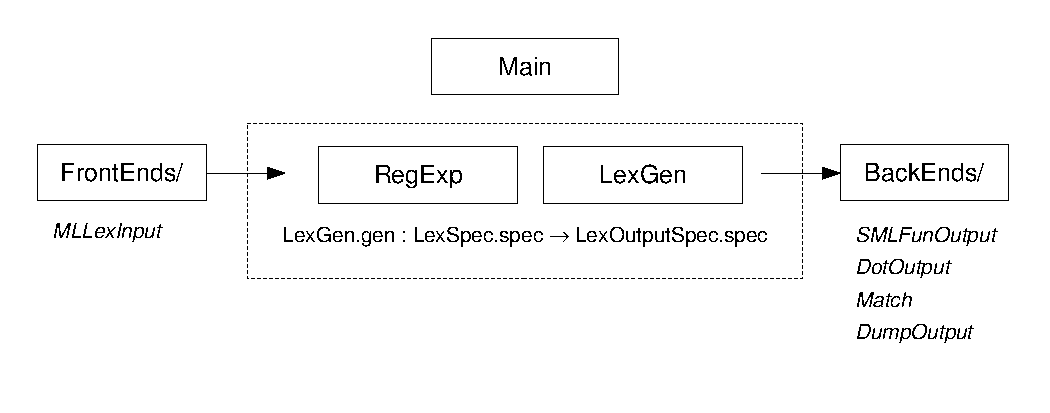
\includegraphics[scale=0.8]{impl-pic.pdf}
\fi
\end{center}
\caption{\ulex{} organization}
\end{figure}

\section{\nm{RegExp}}\label{sec:reg-exp}

In \ulex{}, REs are captured by the abstract type \nm{RegExp.re}.  Introduction
is provided by various ``smart constructors'' (\nm{mkSym}, \nm{mkClosure},
$\dots$), and elimination is provided by the derivatives algorithm.  The
signature for the \rm{RegExp} module is shown below:

\begin{verbatim}
signature REG_EXP =
  sig

    structure Sym : INTERVAL_DOMAIN
    structure SymSet : INTERVAL_SET

    type symbol
    type sym_set
    type re

    val any       : re  (* wildcard *)
    val none      : re  (* EMPTY language *)
    val epsilon   : re  (* the nil character (of length 0) *)

    val mkSym     : symbol -> re
    val mkSymSet  : sym_set -> re

    val mkOr      : re * re -> re
    val mkAnd     : re * re -> re
    val mkXor     : re * re -> re
    val mkNot     : re -> re
    val mkConcat  : re * re -> re
    val mkClosure : re -> re
    val mkOpt     : re -> re
    val mkRep     : re * int * int -> re
    val mkAtLeast : re * int -> re

    val isNone    : re -> bool
    val nullable  : re -> bool
    val derivative : symbol -> re -> re
    val derivatives : re Vector.vector ->
                      ((re Vector.vector) * sym_set) list

    val symToString : symbol -> string
    val toString  : re -> string
    val compare   : re * re -> order

  end
\end{verbatim}

The included structure \nm{SymSet} provides symbol interval sets, which are
ideal when working with dense sets such as unicode character classes.  Interval
set operations (\nm{union}, \nm{complement}, $\dots$) are used extensively;
documentation for the interval set library is available with the SML/NJ
distribution.

Recall that, in using RE derivatives for DFA construction, it is
important to aggresively identify when two REs generate the same
language so that they may be merged to a single state in the automaton.
\nm{RegExp} canonicalizes REs, which is why its \nm{re} type is abstract.
Canonicalization is performed using a lexicographic ordering on REs given by the
\nm{compare} function.  The comparison is lexicographic in the sense that it
first examines the top-level operation of the two REs, and only does more
comparisons if that operation is the same.  We represent REs as follows:
\begin{verbatim}
    datatype re
      = Epsilon
      | Any
      | None
      | SymSet of sym_set
      | Concat of re list
      | Closure of re
      | Op of (rator * re list)
      | Not of re
    and rator = OR | AND | XOR
\end{verbatim}
For the \nm{Op} constructor, which is used for three different commutative
operations, the sub-REs are to be listed in canonical order. The \nm{compare}
function itself will expect that this is the case, and since only smart
constructors can be used to construct REs, the invariant will always hold.

Smart constructors do additional canonicalization beyond ordering.  For
example, \nm{mkNot (mkNot (none))} will be canonicalized
to the same representation as \nm{none}.  Several similar RE equalities
are detected and used.  Also, the smart constructors attempt to push the RE
reprsentation as much toward symbol sets as possible, replacing boolean
operations at the RE level with a single resulting symbol set when possible.
For example, suppose that \nm{AM} held the symbol set for $[A-M]$, \nm{HZ} the
set for $[H-Z]$, and \nm{AZ} the set for $[A-Z]$. Then we would have
\[
\texttt{compare (mkSymSet AZ, mkOr (mkSymSet AM, mkSymSet HZ)) = EQUAL}
\]
The hope is that the cumulative effect of such canonicalization will keep the
generated DFA close to minimal size.

The \nm{derivatve} function constructs a canonicalized derivative for a given
RE with respect to a given symbol; it is a transcription of the algorithm
described in section~\ref{sec:derivatives}.

In general, we will be interested in the derivatives of a vector of REs
(representing the rules in a lexer specification) with respect to \emph{every}
symbol in the alphabet.  As section~\ref{sec:factorings} explains, the unicode
alphabet is too large for us to literally test the derivative at each symbol. 
The \nm{derivatives} function will take a vector of REs and return a list of
\nm{re~Vector.vector~*~sym\_set} \emph{pairs}.  In fact, \nm{derivatives}
is just an implementation of the factor and compress algorithm given
in~\ref{sec:factorings}.  Each pair in the result list represents an arrow
transitioning out of the current state (which corresponds to the input RE
vector) to a new state (the output RE vector) on a given set of symbols (the
output symbol set).  Thus the labor of DFA construction is split between the
\nm{RegExp} module, which computes derivatives (and hence transitions) and
\nm{LexGen}, which actually constructs the DFA graph.

\section{\nm{LexSpec} and \nm{LexOutputSpec}}

Before describing DFA generation, we briefly discuss the relevant input and
output data structures.  The \nm{LexSpec} module has data constructors and
functions relevant to \eg the ML-Lex input specification format, as shown in
Figure~\ref{fig:lex-spec}

\begin{figure}
\begin{verbatim}
    type action = string
    type rule_spec = AtomSet.set option * RegExp.re
    type rule = rule_spec * action

    datatype spec = Spec of {
        decls : string,
        conf : config,
        rules : rule list
      }
\end{verbatim}
\caption{A fragment of \nm{LexSpec}}\label{fig:lex-spec}
\end{figure}

Actions, at least in the present implementation, are just raw strings.  A
\nm{rule} consists of a rule specification and an associated action.  The
optional atom set included with a rule spec represents the start states
to which that rule applies (with \nm{NONE} meaning, strangely enough, all start
states).  With these definitions, a lexer specification is just a list of
rules, some declarations (a raw string containing code) and some miscellaneous
configuration data.

\begin{figure}
\begin{verbatim}
    datatype dfa_state
      = State of {
          id : int,
          label : RegExp.re Vector.vector,
          final : int list,
          next :  (RegExp.sym_set * dfa_state) list ref
        }

    datatype machine = Machine of {
        label : string,
        rules : (RegExp.re * int) vector,
        states : dfa_state list
      }

    type action = string

    datatype spec = Spec of {
        actions : action vector,
        machines : machine list,
        ...  (* configuration data *)
      }
\end{verbatim}
\caption{A fragment of \nm{LexOutputSpec}}\label{fig:lex-output-spec}
\end{figure}

As Figure~\ref{fig:lex-output-spec} illustrates, the output of DFA generation is
\emph{not} a DFA, but a collection of DFAs along with a vector of actions. 
Each \nm{machine} represents a start state for the lexer; that is, each start
state has its own automaton.  However, since start states may use the same
actions, we separate out the actions into a vector so that they are only
emitted once.

A \nm{machine} includes a label, which is just the name of the start state, as
well as the rules relevant to that machine, which are paired with an index to
the associated action in the action vector.  The DFA itself is a list of
states, with the head of the list being $q_0$.  A state, in turn, is labeled by
a vector of REs (with the same length as the \nm{rules} vector in the machine).
 Since a given DFA state may be an accepting state for more than one rule, we
store a \emph{list} of rule indices for the \nm{final} flag.  On a match, the
action for the lowest-index rule is executed first, but that action may use
\nm{REJECT()}, in which case it may be necessary to jump to the action for the
next rule index given in the \nm{final} list.

\section{\nm{LexGen}}\label{sec:lex-gen}

\nm{LexGen} is a very simple module with a single accessible function:
\begin{center}
\nm{gen : LexSpec.spec -> LexOutputSpec.spec}
\end{center}

The first task of the \nm{gen} function is to collate the actions and start
states.  The actions from the input spec are separated from their rules into a
vector.  Afterwards, \nm{gen} iterates over the specified start states,
collecting the rules for each start state and using the \nm{mkDFA} function to
generate a machine for each.

\nm{mkDFA} performs a straightforward imperative DFA construction, using
the \nm{derivatives} function from \nm{RegExp} to compute the transitions out of
each node. A map of RE vectors to DFA nodes is maintained (using
\nm{Vector.collate RegExp.compare} for ordering); this map is used to recognize
when a new out-edge is going to an existing DFA node.  Finally, any transition
to a vector of REs which all generate the empty language is an error transition
(that is, the derivatives for the given transition symbol set all indicate a
non-match).

\section{Front ends}

At the moment, only one front end is available: the ML-Lex specification
format.  Eventually \ulex{} will have its own format.

The ML-Lex front end is fairly straightforward: it uses ML-Yacc to do the
parsing, and can use either ML-Lex or \ulex{} to do the lexing.  The
distribution includes a lexer that was generated from \ulex{} to serve as a
bootstrap.

\section{Back ends}

One exciting aspect of \ulex{} is the ability to easily add back ends.  The
following back ends are currently included in the distribution.

\paragraph{SML control-flow lexer generation}

The most important back end is code generation for SML.  At present, there is a
single code generation strategy: build a lexer using control-flow (\ie
if statements and tail-calls) to match the input.  If the control-flow strategy
turns out to be inadequate, it would be fairly easy to add a code
generator for table-based lexing.

Code generation is performed by expanding stubs in a template SML file.  The
template contains code for dealing with streams and setting up the lexer in the
appropriate way.  Input is read from functional strings, which allow for
the arbitrary lookahead needed for maximal-munch.  These streams also track
the current file position and line number.

A helper module, \nm{ML}, contains a representation for a good portion of the
Standard ML expression langauge, and support for pretty-printing such
expressions.

The generated code includes user actions and the DFA for each start state.
 Within each start state there is one \emph{state function} per DFA node.  Each
state function will examine the next character of input and perform a series of
if-tests to determine the correct transition.  The if-tests perform a
hard-coded binary search over the symbol set intervals for the transitions.

The lexer stores a reference cell for the current functional stream.  Each time
the lexer accepts a token, the cell is updated.  \nm{yytext} is generated (only
when needed) by ``subtracting'' the new stream from the one stored in the
reference cell before updating it.  Subtraction simply rescans the appropriate
number of characters from the stored stream, which should still have the string
in its buffer.

One subtlety is handling calls to \nm{REJECT()}.  Since such calls are fairly
rare, we want to avoid tracking the information \nm{REJECT} needs if it won't
be used.  \nm{REJECT} information consists of (in essence) a list of all the
previous matches.  A previous match could occur on the same DFA state if
multiple REs matched the input at that state; otherwise, the previous match is
a prefix of the \nm{REJECT}ed match.  Whenever a transition is made, the
appropriate previous match information is passed up to the next state. 
However, if the current state is an accepting state that does not use
\nm{REJECT}, then the history is \emph{truncated} at the \nm{REJECT}-free
point, since it could never be used.  This determination is made statically and
is hard-coded into the generated SML lexer.

\paragraph{Graphviz}

The Graphviz toolkit provides easy graph visualization using a very simple
graph description format.  We utilize the DOT format.  The Graphviz backend
will write one DOT file for each start state, showing all nodes for that start
state's DFA, along with labeled transitions.  See \texttt{www.graphviz.org} for
details on the DOT format.

\paragraph{Text dump}

If Graphviz is not available or a more detailed summary is desired, the
\nm{DumpOutput} module can be used to print to standard out every DFA state,
labeled by its RE vector, along with out-edges, for every start state in the
lexer.

\paragraph{Interactive matching}

Finally, a simple interactive back end is available.  Interactive matching
allows a user to enter arbitrary strings and find out (1) if they matched and
(2) what RE matched them.  The code for interactive matching is quite simple.

\section{\nm{Main}}

The \nm{Main} module is the driver for \ulex{}: it is responsible for processing
command-line arguments and hooking up the appropriate front and back ends. 
Since it is very simple, it gives a nice overview of the system and is a good
place to look first in trying to undertand the code.
%		\chapter[\mlantlr]{Implementation: \mlantlr}

%\backmatter

%	\bibliographystyle{plain}
%	\bibliography{deriv.bib}

\end{document}
